\documentclass{article}
\usepackage[utf8]{inputenc}
\usepackage{graphicx}
\usepackage{xcolor}
\renewcommand{\contentsname}{Obsah}
\begin{document}



\centerline{\sc \LARGE Vysoké učení technické v Brně}
\vspace{.5pc}
\centerline{\sc \large Fakulta informačních technologií}

\vspace{5pc}
\centerline{
\includegraphics[scale=.4]{fit}}
\vspace{5pc}

\centerline{\large{\textit{\textbf{Elektronika pro informační technologie}}}}
\vspace{1pc}
\centerline{\large{\textbf{2017/2018}}}

\vspace{5pc}
\centerline{\sc \Large Semestrální projekt}
\vspace{1pc}
\centerline{\sc \large Hynek Bernard}
\centerline{xberna16}
\centerline{20.12.2017}
\clearpage

\tableofcontents
\clearpage
\section{Příklady}
\subsection{Příklad 1, Varianta C}
\vspace{3pc}

\centerline{Stanovte napětí $U_{R_1}$ a proud $ I_{R_1}$. Použijte metodu postupného zjednodušování obvodu}
\vspace{1pc}
\centerline{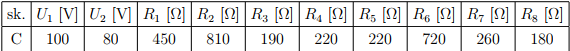
\includegraphics{hodnoty1}}
\vspace{2pc}
\centerline{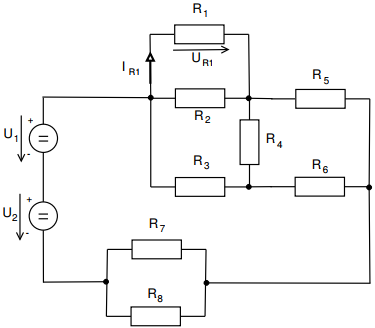
\includegraphics{zadani1}}
\vspace{2pc}




Zapojení postupně zjednodušíme:

\vspace{1pc}

\centerline{$U_{12} = U_1+U_2 = 100+80 = 180 V$}
\centerline{$R_{78} = R_7 \parallel R_8 = \frac{ R_7*R_8}{ R_7+R_8} = \frac{260*180}{260+180} = 106,3636 \Omega$}
\centerline{$R_{12} = R_1 \parallel R_2 = \frac{ R_1*R_2}{ R_1+R_2} = \frac{450*810}{450+810} = 289,2857 \Omega$}


\vspace{2pc}

\clearpage

\noindent Trojúhelník [$R_5 , R_4 , R_6$] převedeme na hvězdu:

\vspace{1pc}

\centerline{$R_A =\frac{ R_4*R_5}{R_4+R_5+R_6} = \frac{220*220}{220+220+720} =41,7241 \Omega$}
\centerline{$R_B =\frac{ R_4*R_6}{R_4+R_5+R_6} = \frac{220*720}{220+220+720} =136,5517 \Omega$}
\centerline{$R_C =\frac{ R_5*R_6}{R_4+R_5+R_6} = \frac{220*720}{220+220+720} =136,5517 \Omega$}

\vspace{2pc}
\noindent Obvod teď vypadá následovně:

\centerline{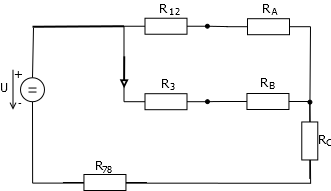
\includegraphics{zjednoduseny1}}


\noindent Dále už jen zjednodušujeme:

\vspace{1pc}
\centerline{$R_{3B}= R_3+R_B = 190+136,5517 = 326,5517 \Omega$}
\centerline{$R_{12A}= R_{12}+R_A = 41,7241+289,2857 = 331,0098 \Omega$}
\centerline{$R_{78C}= R_{78}+R_C = 106,3636+136,5517 = 242,9153 \Omega$}
\centerline{$R_{EKV}= \frac{R_{12A}*R_{3B}}{R_{12A}+R_{3B}}+R_{78C} = \frac{331,0098*326,5517}{331,0098+326,5517}+242,9153 = 407,2981 \Omega$}
\vspace{2pc}
\noindent Když máme $R_{EKV}$ můžeme vypočítat proud v obvodu:

\vspace{1pc}
\centerline{$I = \frac{U}{R_{EKV}} = \frac{180}{407,2981} = 0,4419 A$}
\clearpage

\noindent Nyní můžeme vypočítat napětí a proud na jednotlivých rezistorech a nalézt hledané napětí $U_{R_1}$ a proud $I_{R_1}$ :

\vspace{1pc}
\centerline{$U_{R_{78C}} = R_{78C} *  I = 242,9153*0,4419 = 107,3443 V$}
\centerline{$U_{R_{123AB}} = U - U_{R_{78C}} = 180-107,3443 = 72,6557 V$}
\centerline{$I_{R_{12A}} = \frac{U_{R_{123AB}}}{R_{12A}} = \frac{72,6557}{331,0098} = 0,2195A$}
\centerline{$U_{R_{12}}  = I_{R_{12A}} * R_{12} = 0,2195*289,2857 = \textcolor{red}{63,4982V} = U_{R_1}$}
\centerline{$I_{R_1} = \frac{U_{R_1}}{R_1} = \frac{63,4982}{450} = \textcolor{red}{0,1411A}$}

\clearpage


\subsection{Příklad 2, Varianta H}
\centerline{Stanovte napětí $U_{R_3}$ a proud $I_{R_3}$. Použijte metodu Théveninovy věty.}

\vspace{1pc}
\centerline{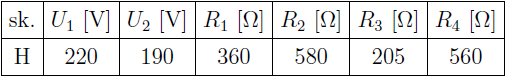
\includegraphics{hodnoty2}}
\vspace{2pc}
\centerline{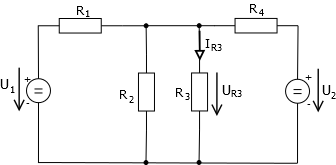
\includegraphics{zadani2}}
\vspace{2pc}

\noindent Odpojíme rezistor $R_3$ podle Theveninova pravidla

\vspace{1pc}
\centerline{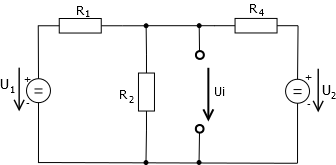
\includegraphics{upraveny2}}
\clearpage
\vspace{2pc}
\noindent Vypočítáme $U_i$, použijeme princip superpozice, nejdříve skratujeme jeden zdroj a poté druhý

\vspace{1pc}


\centerline{$R_2 \parallel R_4 = \frac{ R_2*R_4}{R_2+R_4} = \frac{580*560}{580+560} = 284,9123 \Omega$}
\centerline{$U_{i_1}= U_1 * \frac{R_2 \parallel R_4}{R1+R_2 \parallel R_4} = 220 * \frac{284,9123}{360+284,9123} = 97,1926 V$}
\centerline{$ R_1 \parallel R_2 = \frac{ R_1*R_2}{R_1+R_2} = \frac{360*580}{360+580} = 222,1277 \Omega$}
\centerline{$U_{i_2}= U_2 * \frac{R_1 \parallel R_2}{R4+R_1 \parallel R_2} = 190 * \frac{222,1277}{560+222,1277} = 53,9608 V$}
\centerline{$U_i = U_{i_1}+U_{i_2} = 97,1926+53,9608 = 151,1534V$}
\vspace{2pc}
\noindent Nyní zkratujeme oba zdroje napětí a vypočítáme $R_i$

\vspace{1pc}
\centerline{$R_i = \frac{1}{R_1 \parallel R_2 \parallel R_4} = \frac{1}{\frac{1}{R_1}+\frac{1}{R_2}+\frac{1}{R_4}} =  \frac{1}{\frac{1}{360}+\frac{1}{580}+\frac{1}{560}} = 159,0424\Omega$}
\vspace{2pc}
\noindent Když máme vypočítané $U_i$ a $R_i$, můžeme podle Théveninovy věty vypočítat hledanou hodnotu $I_{R_3}$ a z proudu následně $U_{R_3}$

\vspace{1pc}
\centerline{$I_{R_3} = \frac{U_i}{R_i+R_3} = \frac{151,1534}{159,0424+205} = \textcolor{red}{0,4152A}$}
\centerline{$U_{R_3} = R_3 * I_{R_3} = 205* 0,4152 = \textcolor{red}{85,116V}$}

\clearpage

\subsection{Příklad 3, Varianta A}
\centerline{Stanovte napětí $U_{R_5}$ a proud $I_{R_5}$. Použijte metodu uzlových napětí $(U_A,U_B,U_C)$}

\vspace{1pc}
\centerline{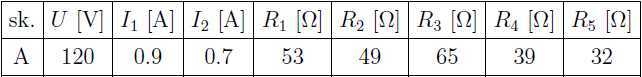
\includegraphics{hodnoty3}}
\vspace{2pc}
\centerline{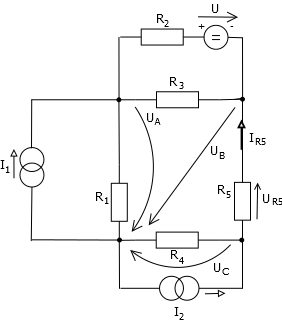
\includegraphics{zadani3}}
\vspace{2pc}

\noindent Sestavíme rovnice pro uzly $A,B,C$ podle I. Kirchhoffova zákona:

\vspace{1pc}
\centerline{$I_1-I_{R_3}-I_{R_1}+I_{R_2}=0$}
\centerline{$I_{R_3}+I_{R_5}-I_{R_2}=0$}
\centerline{$I_2-I_{R_5}-I_{R_4}=0$}
\vspace{2pc}

\noindent Vyjádříme jednotlivé proudy pomocí uzlových napětí:

\vspace{1pc}
\centerline{$I_{R_1}=\frac{U_A}{R_1}=\frac{U_A}{53}$}
\centerline{$I_{R_2}=\frac{U+U_B-U_A}{R_2}=\frac{120+U_B-U_A}{49}$}
\centerline{$I_{R_3}=\frac{U_A-U_B}{R_3}=\frac{U_A-U_B}{65}$}
\centerline{$I_{R_4}=\frac{U_C}{R_4}=\frac{U_C}{39}$}
\centerline{$I_{R_5}=\frac{U_C -U_B}{R_5}=\frac{U_C-U_B}{32}$}
\vspace{2pc}

\noindent Nyní dosadíme proudy do rovnic z prvního kroku

\vspace{1pc}
\centerline{$0,9-\frac{U_A-U_B}{65}-\frac{U_A}{53}+\frac{120+U_B-U_A}{49}=0$}
\centerline{$\frac{U_A-U_B}{65}+\frac{U_C-U_B}{32}-\frac{120+U_B-U_A}{49}=0$}
\centerline{$0,7-\frac{U_C-U_B}{32}-\frac{U_C}{39}=0$}
\vspace{2pc}

\noindent Upravíme na základní tvar

\vspace{1pc}
\centerline{$9227U_A-6042U_B + 0U_C = 565324,5$}
\centerline{$-3648U_A+6833U_B-3185U_C = -249600$}
\centerline{$0U_A-39U_B+71U_C = 873,6$}
\vspace{2pc}

\noindent Sestavíme matici a použijeme cramerovo pravidlo pro výpočet napětí $U_B$ a $U_C$

\vspace{1pc}

\centering {
$$
A =  \left(
 \begin{tabular}{c c c | c}
9227 & -6042 & 0 & 565324,5 \\
-3648 & 6833 &-3185 & -249600 \\
0 & -39 & 71 & 873,6 \\
\end{tabular}
\right)
$$
}
\centering {
$$
detA =  
 \begin{tabular}{|c c c|}
9227 & -6042 & 0  \\
-3648 & 6833 &-3185 \\
0 & -39 & 71 \\
\end{tabular}
= 1765356320
$$
}
\centering {
$$
U_B =  \frac{
 \begin{tabular}{|c c c|}
9227 & 565324,5 & 0  \\
-3648 & -249600 &-3185 \\
0 & 873,6 & 71 \\
\end{tabular}}{detA}
= \frac{8579717328}{1765356320} = 4,86 V
$$
}
\centering {
$$
U_C =  \frac{
 \begin{tabular}{|c c c|}
9227 & -6042 & 565324,5  \\
-3648 & 6833 &-249600 \\
0 & -39 & 873,6 \\
\end{tabular}}{detA}
= \frac{26434144464}{1765356320} = 14,97 V
$$
}

\noindent Z vypočtených napětí $U_B$ a $U_C$ můžeme vypočítat napětí na $R_5$ a následně pomocí ohmova zákona vypočítat proud

\vspace{1pc}
\centerline{$U_{R_5}= U_C-U_B = 14,97-4,86 = \textcolor{red}{10,11V}$}
\centerline{$I_{R_5} = \frac{U_{R_5}}{R_5} = \frac{10,11}{32} = \textcolor{red}{0,3159A}$}



\clearpage
\subsection{Příklad 4, Varianta C}
Pro napájecí napěntí platí: $u_1 = U_1*sin(2\pi f t), u_2 = U_2*sin(2\pi f t)$.\newline
\noindent Ve vztahu pro napětí $u_{C_1} = U_{C_1}*sin(2\pi f t + \varphi_{C_1})$ určete $|U_{C_1}|$ a $\varphi_{C_1}$. 
Použijte metodu smyčkových proudů.


\vspace{1pc}
\centerline{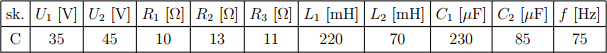
\includegraphics{hodnoty4}}
\vspace{2pc}
\centerline{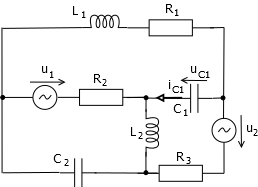
\includegraphics{zadani4}}
\vspace{2pc}


\noindent Vypočítáme úhlovou rychlost $\omega$ z úhlové frekvence $f$

\vspace{1pc}
\centerline{$\omega = 2\pi f = 2\pi*75 = 471,2389rad*s^{-1} $}
\vspace{2pc}

\noindent Vypočítáme Kapacitanci a Induktaci
\centerline{$X_{C_1} = \frac{1}{j*\omega*C_1} = - j\frac{1}{471.2389*0.00023} = -9,2264j\Omega$}
\centerline{$X_{C_2} = \frac{1}{j*\omega*C_2} = - j\frac{1}{471.2389*0.000085} = -24,9655j\Omega$}
\centerline{$X_{L_1} = j*\omega L_1 = j*471,2389*0,22 = 103,6726j\Omega$}
\centerline{$X_{L_2} = j*\omega L_2 = j*471,2389*0,07 = 32,9867j\Omega$}

\clearpage
\noindent Sestavíme rovnice pro napětí ve smyčkách podle II. Kirchhoffova zákona, zavedeme smyčkové proudy $I_A,I_B,I_C$

\vspace{1pc}
\centerline{$I_A : X_{L_1}*I_A+R_1*I_A+X_{C_1}*(I_A*I_C)+R_2*(I_A-I_B)-U_1=0$}
\centerline{$I_B : R_2*(I_B-I_A) +X_{L_2}*(I_B+I_C)+X_{C_2}*I_B+U_1=0$}
\centerline{$I_C : X_{C_1}*(I_C+I_A)+X_{L_2}*(I_C+I_B)+R_3*I_C-U_2=0$}
\vspace{2pc}

\noindent Sestavíme matici a vypočteme $I_A$ a $I_C$

\centering {
$$
A =  \left(
\begin{tabular}{c c c | c}
$R_1+R_2 + X_{L_1}+X_{C_1}$ & -$R2$ & $X_{C_1}$ & $ U_1$ \\
$-R_2$ & $R_2+X_{L_2}+X_{C_2}$ & $X_{L_2}$ & $-U_1$ \\
$X_{C_1}$ & $X_{L_2}$ & $X_{C_1}+X_{L_2}+R_3$ & $U_2$ \\
\end{tabular}
\right)
$$
}
\centering {
$$
A =  \left(
\begin{tabular}{c c c | c}
$10+13+103,6726j-9,2264j$ & $-13$ & $-9,2264j$ & $ 35$ \\
$-13$ & $13+32,9867j-24,9655j$ & $32,9867j$ & $-35$ \\
$-9,2264j$ & $32,9867j$ & $-9,2264j+32,9867j+11$ & $45$ \\
\end{tabular}
\right)
$$
}
\centering {
$$
A =  \left(
\begin{tabular}{c c c | c}
$23+94,4462j$ & $-13$ & $-9,2264j$ & $ 35$ \\
$-13$ & $13+8,0212j$ & $32,9867j$ & $-35$ \\
$-9,2264j$ & $32,9867j$ & $11+23,7603j$ & $45$ \\
\end{tabular}
\right)
$$
}
\centering {
$$
detA =  
\begin{tabular}{|c c c|}
$23+94,4462j$ & $-13$ & $-9,2264j$ \\
$-13$ & $13+8,0212j$ & $32,9867j$ \\
$-9,2264j$ & $32,9867j$ & $11+23,7603j$ \\
\end{tabular}
= -22239,2839 + 104075,7145j
$$
}
\centering {
$$
I_A =  \frac{
\begin{tabular}{|c c c|}
$35$ & $-13$ & $-9,2264j$ \\
$-35$ & $13+8,0212j$ & $32,9867j$ \\
$45$ & $32,9867j$ & $11+23,7603j$ \\
\end{tabular}}{ -22239,2839 + 104075,7145j}
= -0,1336 - 0,1389j
$$
}
\centering {
$$
I_C =  \frac{
\begin{tabular}{|c c c|}
$23+94,4462j$ & $-13$ & $35$ \\
$-13$ & $13+8,0212j$ & $-35$ \\
$-9,2264j$ & $32,9867j$ & $45$ \\
\end{tabular}}{-22239,2839 + 104075,7145j}
= 0,9647+1,1378j
$$
}
\vspace{2pc}
\noindent Z vypočítaného proudu můžeme vypočítat hledané hodnoty $|U_{C_1}|$ a $\varphi_{C_1}$

\vspace{1pc}
\centerline{$U_{C_1}=(I_C+I_A)*X_{C_1} = (0,9647+1,1378j -0,1336 - 0,1389j) *  -9,2264j = 9,2163-7,6681jV$}
\centerline{$|U_{C_1}|=\sqrt{9,2163^2-7,6681^2}=\textcolor{red}{68,0161V}$}
\centerline{$\varphi_{C_1} = arctg(\frac{-7,6681}{9,2163}) = \textcolor{red}{-0,694rad}$}
\clearpage
\subsection{Příklad 5, Varianta H}

\clearpage

\section{Výsledky}
\begin{tabular}{|c|c|l|}
\hline
Příklad & Zadání & Výsledek \\ \hline
1 & C & $I_{R_1} = 0,1411A, U_{R_1} = 63,4982V$ \\ \hline
2 & H & $I_{R_3} = 0,4152A, U_{R_3} = 85,116V$ \\ \hline
3 & A & $I_{R_5} = 0,3159A, U_{R_5} = 10,11V$ \\ \hline
4 & C & $|U_{C_1}|=68,0161V, \varphi_{C_1}= -0,694rad$ \\ \hline 
5 & H & xxx \\ \hline
\end{tabular}

\end{document}